\documentclass{article}

\usepackage{color}
\usepackage{amsmath}
\usepackage{fullpage}
\usepackage{multirow}
\usepackage{graphicx}
\usepackage{pdfpages}


\sloppy
\definecolor{lightgray}{gray}{0.5}
\setlength{\parindent}{0pt}
\renewcommand{\arraystretch}{1.2}

\newcommand{\tab}{\hspace{20 mm}}

% part numbering command
\newcounter{partNum}
\newcommand{\partNum}{%
        \stepcounter{partNum}%
        \thepartNum}
\newcommand{\sectPart}[1]{\section*{Part \partNum: #1}}

\newcommand{\bitem}[1]{\item \textbf{#1}}

\newcommand{\assignment}{PreLab 11}
\newcommand{\duedate}{April 18, 2014}
\newcommand{\header}{\noindent \textbf{ECE348 \assignment, Spring 2014 \\
					 Group C1 \\ 
					 Spencer Barton sebarton \\
					 \duedate} \vspace{0.10in} \hrule}

\begin{document}
    
%=======================================================

\header

%=======================================================

\sectPart{Description}

\paragraph*{}
We plan to build an RTOS. We will implement priority ceiling with mutex and a timer to handle periodic tasks. A serial buffer shall act as a shared resource for the mutex. We shall use serial to output details on current tasks and the state of the various tasks. Two interrupts that we will use are swi (for yield) and timer. If we have time we will also implement yield.	

\paragraph*{}
We shall include the following items:
\begin{enumerate}
\item Serial Communications
\item Counter / timer
\item Mutex
\item Priority Ceiling
\item Watchdog
\end{enumerate}

\paragraph*{}
Our interrupts will be:
\begin{enumerate}
\item Timer interrupt
\end{enumerate}

%-----------------------------------------
\sectPart{Requirements}

\begin{enumerate}
\bitem{System Inputs}
	\begin{enumerate}
	\bitem{mutexDisableBtn} Boolean based off of button on board (PB1). When asserted this button disables mutex. Default state is unasserted.
	\bitem{taskEnableBtn[0:2]} Boolean based off of SW[0:2]. When asserted this switch enables a task. When off the task is disabled.
	\end{enumerate}
\bitem{System Outputs}
	\begin{enumerate}
	\bitem{Serial} The Scheduler shall expose internal task state via serial. It shall write to serial after each scheduling event. The format shall be as follows:
\begin{verbatim}
 Task(Default Priority) | Priority | Running | Ready to Run | Scheduled to Run
 -----------------------+----------+---------+--------------+-----------------
 1                      | 1        | false   | true         | false
 3                      | 0        | true    | false        | true
 5                      | 5        | true    | false        | false
\end{verbatim}
	\end{enumerate}
\bitem{State Variables}
	\begin{enumerate}
	\bitem{mutexEnabled} Boolean state variable to keep track of mutex state.
	\end{enumerate}
\bitem{Requirements}
	\begin{enumerate}
	\item When mutexDisableBtn button is pressed the mutex shall be disabled with the mutex enabled otherwise.
	\item When the SWx switch is on task x shall be enabled and when the switch is off task x shall be disabled.
	\item When the scheduler completes execution it shall write the current task state to serial.
	\item Scheduler shall at least every .1 second.
	\item Poll Button Task shall occur every .5 second.
	\item Watchdog Kick Task shall occur every .5 second.
	\item Short Block Task shall occur with period of 2 seconds and will run for .1 seconds with a blocking time of .1 seconds (holding the mutex).	
	\item Long Block Task shall occur with period of 1.9 seconds and will run for .3 seconds with a blocking time of .3 seconds (holding the mutex).
	\item When Long Task and Short Task are enabled both shall attempt to acquire the mutex with Long Task periodically acquiring the mutex first and rising above Short Task in priority due to priority ceiling.
	\item RTOS shall start with mutexs enabled and shall initialize tasks before running.
	\end{enumerate}
\end{enumerate}

%-----------------------------------------

\sectPart{State Chart}

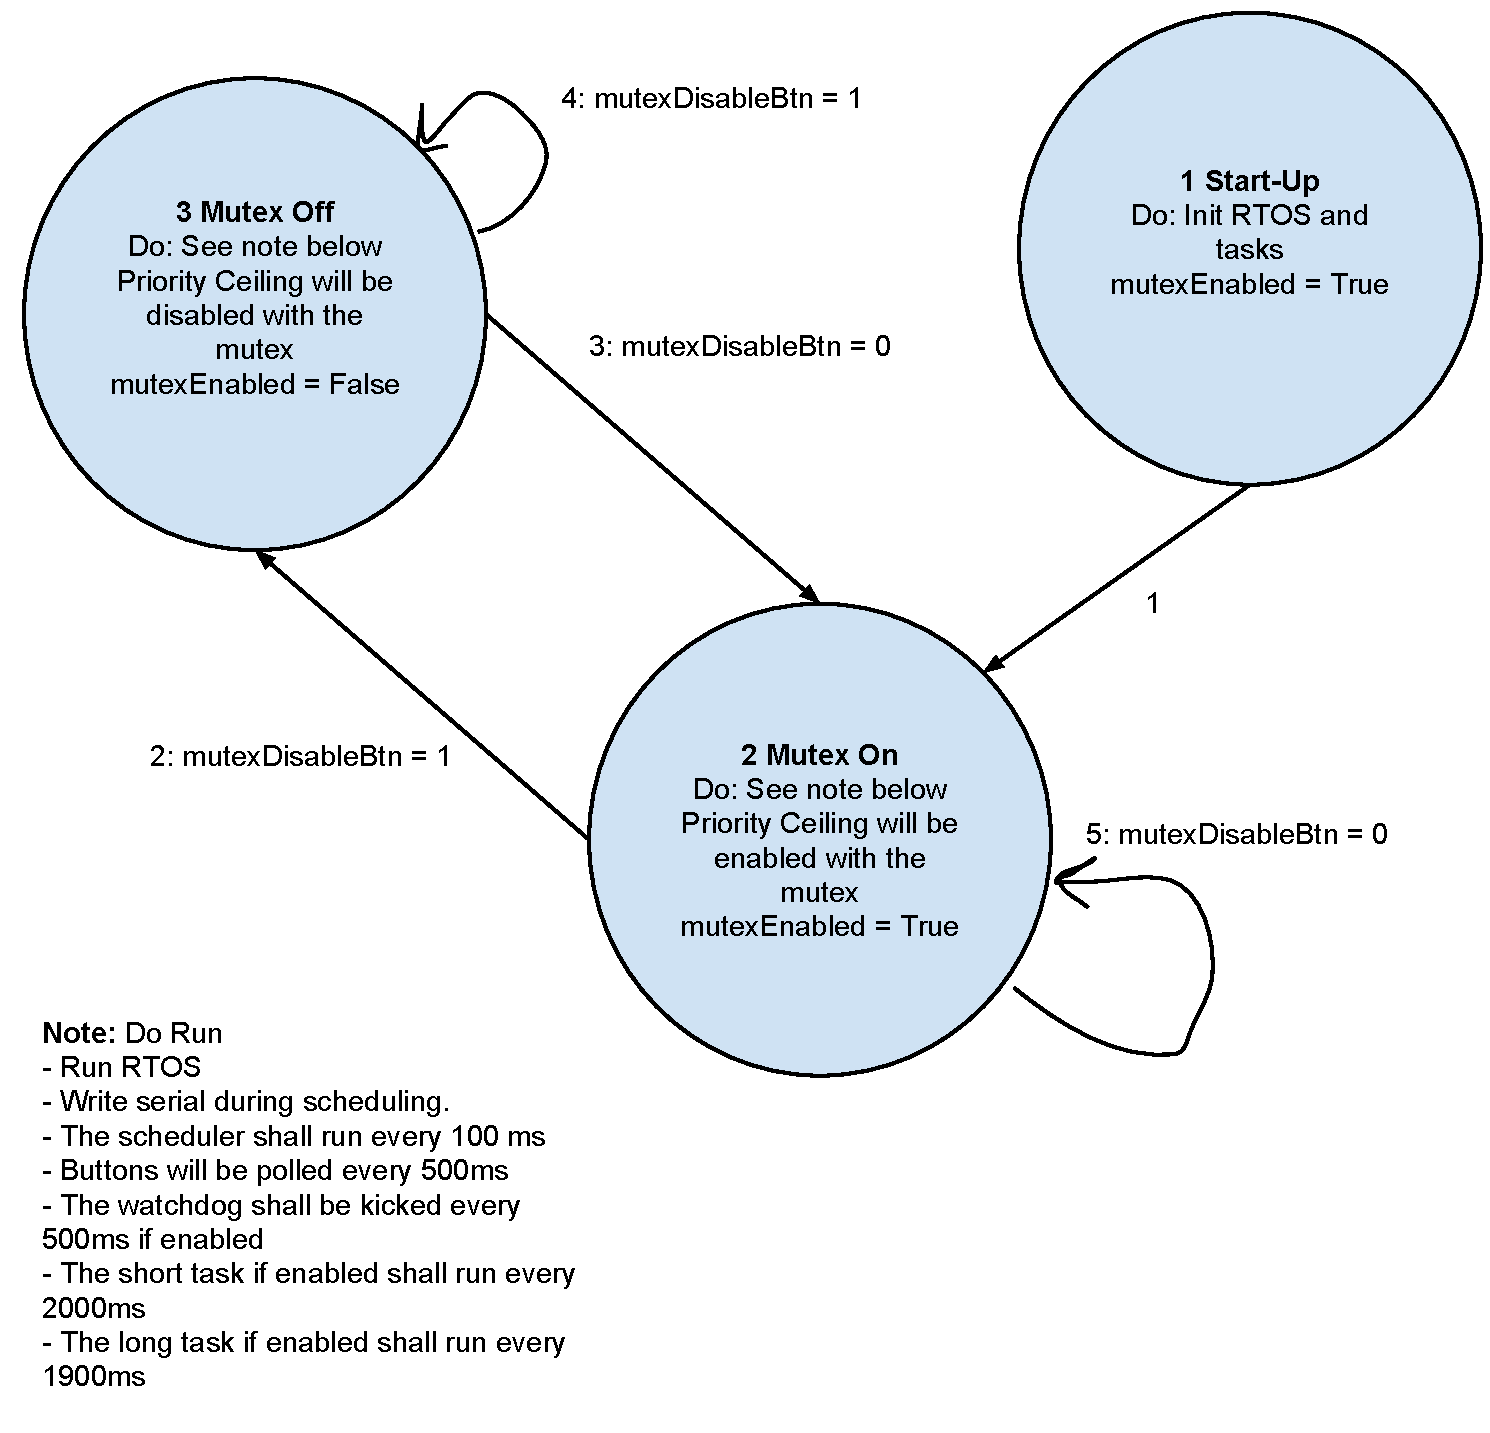
\includegraphics[scale=.5]{RTOS_State_Chart.pdf}

\sectPart{Requirements/State-Chart Traceability Table}

NOTE: Because we are implementing an RTOS that majority of our requirements relate to RTOS timing and behavior. RTOS state is not easily encapsulated in a state diagram as its state is based on task timing. The state transition diagram relates to the demonstration and peripherals which function as a result of correct RTOS behavior but do not define the RTOS behavior itself.

\vspace*{1em}

\begin{tabular}{c | c | c | c | c | c | c | c | c}
Req. & State 1 & State 2 & State 3 & Trans 1 & Trans 2 & Trans 3 & Trans 4 & Trans 5 \\ \hline
a & - & X & X & - & X & X & X & X \\
b & - & - & - & - & - & - & - & - \\
c & - & X & X & - & - & - & - & - \\
d & - & - & - & - & - & - & - & - \\
e & - & - & - & - & - & - & - & - \\
f & - & - & - & - & - & - & - & - \\
g & - & - & - & - & - & - & - & - \\
h & - & - & - & - & - & - & - & - \\
i & - & - & - & - & - & - & - & - \\
j & X & - & - & X & - & - & - & - \\
\end{tabular}

%-----------------------------------------

\sectPart{Scheduling}

Connor

%-----------------------------------------

\sectPart{Watchdog/COP}

Connor

%-----------------------------------------

\sectPart{Test Plan}

\subsection*{Part 7.1: White Box Testing}

NOTE: Key used to simplify table: M is mutexDisableBtn = 1 and ~M is mutexDisableBtn = 0

\vspace*{2em}

\textbf{Tests}\\
\begin{tabular}{c | c | c | c | c | c | c}
Test & Init State & In1 & In2 & In3 & In4 & In5 \\ \hline
1 & 1 & Any(2) & ~M(2) & M(3) & M(3) & ~M(2) \\
\end{tabular}

\vspace*{2em}

\textbf{Traceability} \\
\begin{tabular}{c | c | c | c | c | c}
Test & Trans 1 & Trans 2 & Trans 3 & Trans 4 & Trans 5 \\ \hline
1 & X & X & X & X & X \\
\end{tabular}

\subsection*{Part 7.2: Black Box Testing}

\textbf{Tests}\\
\begin{tabular}{c | c{30em} }
Test & Description \\ \hline
\end{tabular}

\vspace*{2em}

\textbf{Traceability} \\
\begin{tabular}{c | c | c | c | c | c}
Test & Trans 1 & Trans 2 & Trans 3 & Trans 4 & Trans 5 \\ \hline
1 & X & X & X & X & X \\
\end{tabular}

%-----------------------------------------

\sectPart{Hardware}

Connor

%-----------------------------------------

\sectPart{Acceptance Test Plan}

Connor

%-----------------------------------------

\section*{Appendix}

	\subsection*{RTOS API}
		TODO
		
%=======================================================

\end{document}
